\begin{center}
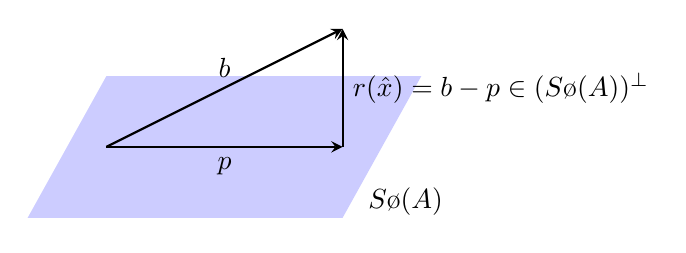
\begin{tikzpicture}
	\tikzset{>=stealth}
	\fill[blue!20] (0,0) -- (1,1.8) -- (5,1.8) -- (4,0) -- cycle;

	\node (sa) at (4.8,0.2) {$S\text{ø}(A)$};
	
	\draw[thick,->] (1,0.9) to node[below]{$p$} (4,0.9);
	\draw[thick,->] (1,0.9) to node[above]{$b$} (4,2.4);
	\draw[thick,->] (4,0.9) to node[right]{$r(\hat{x})=b-p\in 
		(S\text{ø}(A))^\bot$} (4,2.4);
\end{tikzpicture}
\end{center}
